\documentclass[12pt,letterpaper,titlepage,en-US]{article}

\usepackage{basicstyle}
\usepackage{report}
\usepackage{knit}
\usepackage{amsmath}
\usepackage{xcolor}
\usepackage{listings}
\usepackage{fancyvrb}
\usepackage{graphicx}
\definecolor{lbcolor}{rgb}{0.969, 0.969, 0.969} 

 \lstset{ 
    language=Java, % choose the language of the code
    basicstyle=\fontfamily{pcr}\selectfont\footnotesize\color{black},
    keywordstyle=\color{black}\bfseries, % style for keywords
    numbers=none, % where to put the line-numbers
    numberstyle=\tiny, % the size of the fonts that are used for the line-numbers     
    backgroundcolor=\color{lbcolor},
    showspaces=false, % show spaces adding particular underscores
    showstringspaces=false, % underline spaces within strings
    showtabs=false, % show tabs within strings adding particular underscores
    frame=single, % adds a frame around the code
    tabsize=2, % sets default tabsize to 2 spaces
    rulesepcolor=\color{gray},
    rulecolor=\color{black},
    captionpos=b, % sets the caption-position to bottom
    breaklines=true, % sets automatic line breaking
    breakatwhitespace=false, 
}


\newcommand{\hmwkTitle}{Mini Project \#3}
\DTMsavetimestamp{DueDate}{2019-03-07T10:00:00-06:00}
\newcommand{\hmwkClass}{CS 6313.001}
\newcommand{\hmwkClassName}{Statistical Methods for Data Science}
\newcommand{\hmwkClassInstructor}{Instructor: Prof. Min Chen}
\newcommand{\hmwkAuthorName}{Shyam Patharla}
\newcommand{\hmwkAuthorNetID}{sxp178231}

\newcommand{\hmwkAuthorOneName}{Lizhong Zhang (lxz160730) : P1(ae), P2(bcde)}
\newcommand{\hmwkAuthorTwoName}{Hanlin He (hxh160630) : P1(bcd), P2(af)}



%
% Title Page
%

\title{
    \vspace{1in}
    \textmd{\textbf{\hmwkClassName \\\hmwkClass:\ \hmwkTitle }}\\
     \normalsize\vspace{0.1in}\small{Due\ on\ \DTMusedate{DueDate}\ at \DTMusetime{DueDate} }\\
    \vspace{0.1in}\large{\textit{\hmwkClassInstructor}}\\
    \vspace{0.5in}
\includegraphics[height=2.4em]{UTD_logo_BW}\\
    \vspace{2in}
}

\author{\textbf{\hmwkAuthorName\ \footnotesize{(\hmwkAuthorNetID)}} \\ }
\date{}
\makeindex

\begin{document}
\maketitle

\pagenumbering{Roman}

\tableofcontents

\pagebreak
\pagenumbering{arabic}


\section{Answers}

\subsection{}

\subsubsection{Compute the mean squared error of an estimator using Monte Carlo simulation}
Given: n, $\theta$, nsim

\begin{enumerate}
 
\item First, we generate a sample of size n from the uniform distribution in the interval \textbf{(0, $\theta$}). 

\item We replicate Step 1 for \textbf{nsim} times and store the values of the nsim samples in a vector called \textbf{data}.

\item To get the maximum likelihood estimators for each of these nsim samples, we take the mean of each column in the vector \textbf{data}. We store this in a vector \textbf{mle.est}. 

\begin{knitrout}
\definecolor{shadecolor}{rgb}{0.969, 0.969, 0.969}\color{fgcolor}
\begin{kframe}
\begin{verbatim}
>  mle.est <- apply(data,2,max)
\end{verbatim}
\end{kframe}
\end{knitrout}


\item We get the estimator mean squared error using the formula:

\begin{knitrout}
\definecolor{shadecolor}{rgb}{0.969, 0.969, 0.969}\color{fgcolor}
\begin{kframe}
\begin{verbatim}
> result1 <- sum((mle.est-theta)^2)/rep
\end{verbatim}
\end{kframe}
\end{knitrout}



\item To get the method of moments estimators for each of these nsim samples, we take the mean of each row in the vector \textbf{data} and multiply it by 2. We store this in a vector \textbf{mom.est}. 

\begin{knitrout}
\definecolor{shadecolor}{rgb}{0.969, 0.969, 0.969}\color{fgcolor}
\begin{kframe}
\begin{verbatim}
>  mom.est <- apply(data,2,max)
\end{verbatim}
\end{kframe}
\end{knitrout}


\item We get the estimator mean squared error using the formula:

\begin{knitrout}
\definecolor{shadecolor}{rgb}{0.969, 0.969, 0.969}\color{fgcolor}
\begin{kframe}
\begin{verbatim}
> result1 <- sum((mom.est-theta)^2)/rep
\end{verbatim}
\end{kframe}
\end{knitrout}
\end{enumerate}


\subsubsection{For a given combination(n, theta), compute the mean squared errors of estimators obtained using maximum likelihood estimation and method of moments}
\begin{knitrout}
\definecolor{shadecolor}{rgb}{0.969, 0.969, 0.969}\color{fgcolor}
\begin{kframe}
\begin{verbatim}
# Let n=5, theta=50,rep=1000
> compare.est(5,50,1000)
# [1] 120.4905 674.0310
\end{verbatim}
\end{kframe}
\end{knitrout}


The first element of the result array is the mean squared error for the estimator obtained using maximum likelihood estimation. The second is for the one obtained using the method of moments.\\

The error for the estimator obtained using method of moments is significantly higher compared to its MLE counterpart.


\subsubsection{Repeat part (b) for the remaining combinations of (n, theta) and summarize your results graphically}
\begin{table}[H]
\centering
\begin{tabular}{|c|c|c|c|c|}
\hline
& $\theta=1 $  &$\theta=5 $   &$\theta=50$    &$\theta=100$ \\\hline
n=1	&0.339195 	 &7.703114 	&811.1820	 &3311.070\\\hline
n=2	&	0.1621363 	&4.434155 	&419.0197 	&1784.770\\\hline
n=3	&0.09695403 	&2.431108	 &262.1221 	&921.4235\\\hline
n=5	&0.05210957 	&1.160537	 &120.4905 	&462.295\\\hline
n=10	&0.01460649 	&0.4167772	 &35.15594	& 155.2607\\\hline
n=30	&0.001593959 	&0.04953917	 &4.541694 	&20.21065\\\hline
\end{tabular}
\caption{Mean Squared Error for Maximum Likelihood Estimator}\label{1}
\end{table}


\begin{table}[H]
\centering
\begin{tabular}{|c|c|c|c|c|}
\hline
& $\theta=1 $  &$\theta=5 $   &$\theta=50$    &$\theta=100$ \\\hline
n=1	&0.320539 	 &7.841863 	& 816.5786   &3265.399\\\hline
n=2	&	0.2893060 	&7.506875	&734.2253	&3041.526\\\hline
n=3	&0.27582063 	&6.867733	 &689.8118 	&2687.4609\\\hline
n=5	&0.27065755 	&6.642441	 &674.0310	&2630.757\\\hline
n=10	&0.25359251 	&6.5436014	 &641.09682	& 2572.9569\\\hline
n=30	&0.252542160 	&6.23571907	 &634.189762 	&2516.58880\\\hline
\end{tabular}
\caption{Mean Squared Error for Method of Moments Estimator}\label{1}
\end{table}


Conclusions:
\begin{enumerate}
\item For a fixed value of n, the mean squared error increases with $\theta$ for both MLE and MOM estimators.
\item For a fixed value of $\theta$, the mean squared error decreases with n for both MLE and MOM estimators.
\item For a given (n,$\theta$),the error for the estimator obtained using method of moments is significantly higher compared to its MLE counterpart.
\end{enumerate}
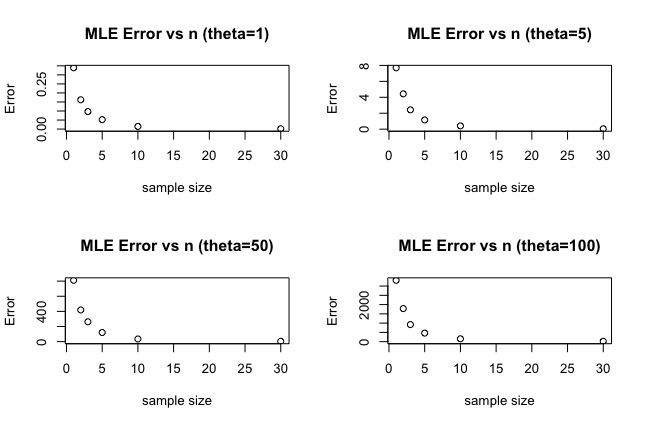
\includegraphics[scale=0.6]{graph1.jpeg}\\
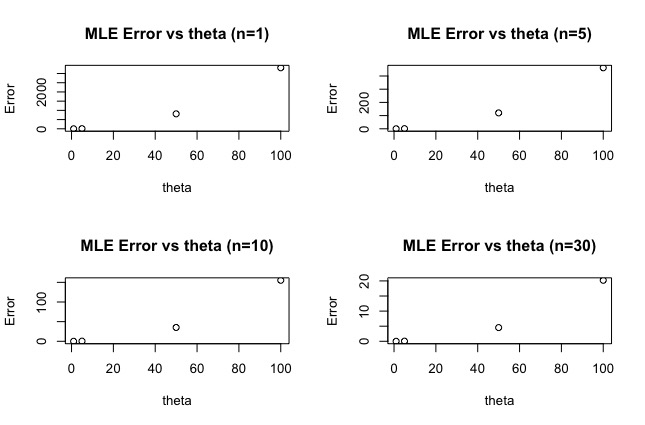
\includegraphics[scale=0.6]{graph2.jpeg}\\

Similar characteristics exist for the method of moments estimator.

\subsubsection{Which estimator is better?}
The \textbf{maximum likelihood estimator} is clearly better for our problem irrespective of n or $\theta$ because the errors are less than thos of there Method of Moments counterparts for all $(n,\theta).$

\subsection{}
\subsubsection{Derive an expression for the maximum likelihood estimator of theta}
We have:
\begin{equation}
f(x) = \begin{cases}\frac{ \theta}{ x^{\theta+1}}, x\geq1
\\ 0, x<1 \end{cases}
\end{equation}




\begin{equation}
ln f(X) = ln f(X_{1}, X_{2},...X_{n})= ln \prod_{i=1}^{n}f(X_{i})
\end{equation}

\begin{equation}
ln f(X) =  \sum_{i=1}^{n} ln f(X_{i})
\end{equation}

\begin{equation}
ln f(X) = \sum_{i=1}^{n}ln(\frac{\theta}{x^{\theta+1}})
\end{equation}

\begin{equation}
ln f(X) = \sum_{i=1}^{n}(ln(\theta) - (\theta+1) ln(X_{i}))
\end{equation}

\begin{equation}
ln f(X) =nln(\theta) -  \theta\sum_{i=1}^{n}ln(X_{i})  - \sum_{i=1}^{n}ln(X_{i})
\end{equation}
Taking the derivative and equating it to 0, we get:
\begin{equation}
\frac{\partial ln f(X)}{\partial \theta} =0
\end{equation}

\begin{equation}
\frac{n}{\hat{ \theta}}-\sum_{i=1}^{n}ln(X_{i}) =0
\end{equation}

\begin{equation}
\hat{\theta}=\frac{n}{\sum_{i=1}^{n}lnf(X_{i})}
\end{equation}


\subsubsection{Calculate an estimate for theta for the given data}
We have:\\
$
X_{1}=21.72, X_{2}=14.65, X_{3}=50.42 \\
X_{4}=28.78, X_{5}=11.23\\
n=5\\
$
Substituting $X_{1},X_{2},X_{3},X_{4},X_{5}$ and n, we get:
\begin{equation}
\hat{\theta}=0.323394
\end{equation}


\subsubsection{Obtain the estimate by numerically maximizing log-likelihood function in R}
We first write the negative log likelihood function:
\begin{knitrout}
\definecolor{shadecolor}{rgb}{0.969, 0.969, 0.969}\color{fgcolor}
\begin{kframe}
\begin{verbatim}
neg.loglik.fun <- function(par,dat)
{ 
  result <- NROW(dat)*log(par) - (par+1)*sum(log(dat))
  return(-1*result)
}
\end{verbatim}
\end{kframe}
\end{knitrout}



We then run the \textbf{optim} function to find the value of $\theta$ where the negative log likelihood function has the minimum value:
\begin{knitrout}
\definecolor{shadecolor}{rgb}{0.969, 0.969, 0.969}\color{fgcolor}
\begin{kframe}
\begin{verbatim}
> ml.est <- optim(par=c(0.1), fn=neg.loglik.fun, 
method = "L-BFGS-B",lower=rep(0.005), hessian=TRUE, dat=data)

> ml.est
$par
[1] 0.3233885

$value
[1] 26.10585

$counts
function gradient 
       9        9 

$convergence
[1] 0

$message
[1] "CONVERGENCE: REL_REDUCTION_OF_F <= FACTR*EPSMCH"

$hessian
         [,1]
[1,] 47.81116
\end{verbatim}
\end{kframe}
\end{knitrout}
The value of 0.3233885 obtained is very close to the manually calculated value of $\hat{\theta
}=0.3234.$


\subsubsection{Provide a standard error and a 95 percent confidence interval for theta}
The standard error is given by:
\begin{knitrout}
\definecolor{shadecolor}{rgb}{0.969, 0.969, 0.969}\color{fgcolor}
\begin{kframe}
\begin{verbatim}
# Calculating the standard error
> (0.3233885-0.323394)^2
# [1] 3.025e-11

> sqrt(3.025e-11)
# [1] 5.5e-06
\end{verbatim}
\end{kframe}
\end{knitrout}


\begin{knitrout}
\definecolor{shadecolor}{rgb}{0.969, 0.969, 0.969}\color{fgcolor}
\begin{kframe}
\begin{verbatim}
> conf.int(0.3233885,5.5e-06,20,0.05)
# [1] 0.3233860 0.3233908
\end{verbatim}
\end{kframe}
\end{knitrout}


We repeat the process to get many confidence intervals.
\begin{knitrout}
\definecolor{shadecolor}{rgb}{0.969, 0.969, 0.969}\color{fgcolor}
\begin{kframe}
\begin{verbatim}
> nsim<-1000
> ci.mat<-replicate(1000,conf.int(0.3233885,5.5e-06,20,0.05))
\end{verbatim}
\end{kframe}
\end{knitrout}

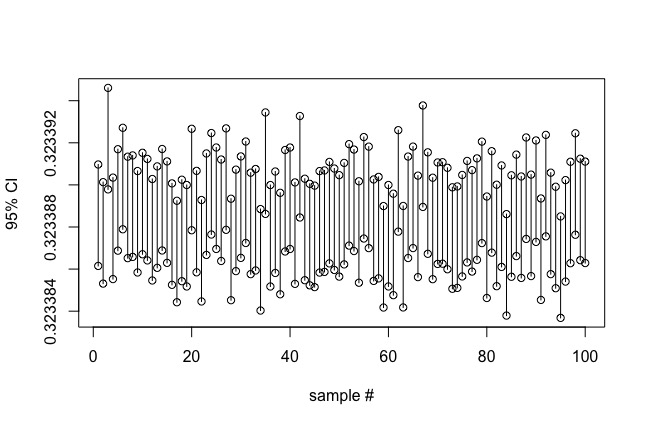
\includegraphics[scale=0.6]{ci.jpeg}\\
The confidence intervals seem to give us a good idea of where $\theta$ lies.
\section{R Code}
\lstinputlisting{/users/psprao/downloads/stats/R-code/project3/Q1.R}
\lstinputlisting{/users/psprao/downloads/stats/R-code/project3/Q2.R}


\end{document}
